\chapter{Conclusion}
\label{chap:conclusion}

\itquote[0mm]{
Shoot for the moon. Even if you miss, you'll land among the stars.
}{B. Littrell}

\section{Summary}
%\label{sec:conclusion.summary}

This thesis describes how a combination of several strategies for easier learning and
supporting motivation, together with the adaptivity of the system
through techniques of artificial intelligence,
can lead to an efficient learning of introductory programming. % too strong?
Creating such a system is, however, not a one-shot task, but rather a long series
of small iterative improvements of a programming game, user interface,
domain, student and tutor models, and the analysis layer.
We have already completed a few iterations of improvements with
% our adaptive learning system for introductory programming,
RoboMission,
tested its usability in schools during an Hour of Code,
as well as in two competitions for primary and secondary school students,
% (Purkiada, Sob 2018) Sob - consider including a photo
and published our initial research on programming tasks similarities \cite{alg.similarity},
and on the adaptive approach to learning programming \cite{robomission}.

% \imgW[0.7]{intersob}{InterSoB ... (Photo by Vendula Němcová.}

% \section{Lessons Learned}

\section{Future Work}
%\label{sec:conclusion.future-work}

Many improvement iterations are yet to be undertaken. After adding
new game elements and programming concepts (e.g. functions and compound
conditions), it will possible to create more advanced problem sets,
and extend the use
case of the system beyond the short hour motivational tutorial (\emph{Hour of Code mode}).  % grammar
In \emph{foundations mode}, students could spend from a few days to several weeks practicing
programming, transitioning gradually from block-based to textual programming
in RoboCode.
% missions for learning new programming elements, esp. functions and compound conditions
% Usage: for a standard primary-secondary school programming curriculum.
Then, in \emph{university mode} targeting at high school and university students,
tasks would teach programming in Python, and possibly even advanced algorithmic
concepts (\cref{fig:robomission-search-tree}).
% at home / secondary schools, KSI (0th problem set), IB111 (0th/1st motivational lesson)
Furthermore, we would like to introduce a \emph{competition mode}, for
straightforward usage of new tasks in a programming contest,
leaving these problem sets public for everybody for practice once the
competition is over.
% Competitions --  (both blocks and Python depending on the competition) such as Purkiada, Pevnost FI, KSI, InterLos, InterSob, new FIBot (new problem sets -> public for everybody for practice after the competition; %this also includes testing mode for RH interns
% 5. Cooperation: multiplayer programming game

\begin{figure}[htb]
\centering
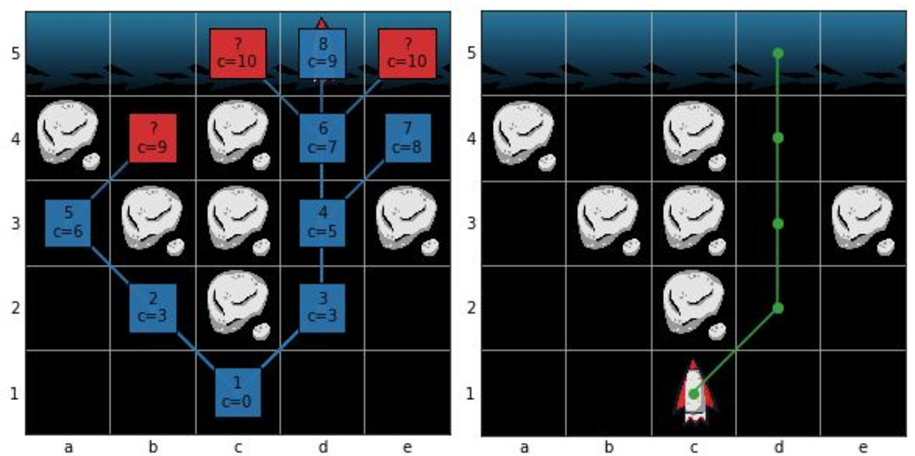
\includegraphics[width=\textwidth]{img/robomission-search-tree}
\caption{%
  Example of how the Space World can be used for learning algorithms,
  in this case Dijkstra's shortest path algorithm
  (used at a workshop for high school students).}
\label{fig:robomission-search-tree}
\end{figure}

In addition to new problem sets, we plan to implement a real-time dashboard for teachers,
which would visualize progress and estimated skills of students and suggest
which students needs a help right now, and possibly even how to pair students
for efficient pair programming.

With growing content, it would become useful to build more complex
domain, student and tutor models. In order to add overlapping concepts
into the domain and use them to more accurately predict student performance,
we need to analyze how multiple skills interact in a single
task to produce the final performance. %, in order to predict performance.
% in a single task. % to produce a single performance.
Using data from a single task session,
we want to detect which concepts contained in the task
is the student struggling with.
Models might be further improved by including uncertainty of estimates,
forgetting of skills, and planning of tutor actions.

To evaluate which versions of models increase the quality of the system,
analysis layer should be extended to allow for AB experiments
% In addition to compare several versions of student or tutor models,
% ... experiment on block-based vs text-based programming
and a careful attention should be paid to both long-term and
online attributable metrics.
% TODO: Reformulate.
Unbiased evaluation is complicated by feedback loops caused by the fact, that
the collected data on which the system is evaluated are influenced by the
adaptive behavior of the system.
% and long-term metrics monitoring, simulated experiments
In order to further align measured metrics with the system mission,
we can explore how to reduce noise in flow observations
by combining subjective user feedback with objective performance measures.
Having a reliable flow observations would be a great step towards optimizing
the total amount of time spent in the state of flow.

%- peer tutoring (in a classroom)
% - if RL approaches can help
